\newcommand\toplisting[0]{\hrule\vspace{5pt}}
\newcommand\bottomlisting[0]{\vspace{4pt}\hrule}

\newcommand\customlisting[5]{
  \begin{figure}[#1]
    \centering
    \begin{minipage}{#3\linewidth}
      \toplisting
      \lstset{caption=#4,label=#2}
      \input{../#5}
      \bottomlisting
    \end{minipage}
  \end{figure}
}

\newcommand\transportInterface[1]{
  \begin{figure}[t]
    \centering
    \begin{minipage}{0.8\linewidth}
      \toplisting
      \input{../transport/transport/core/src/main/scala/transport/Transport.listings}
      \lstset{caption=#1,label=transportInterface}
      \input{../transport/transport/core/src/main/scala/transport/package.listings}
      \bottomlisting
    \end{minipage}
  \end{figure}
}

\newcommand\actorWrapper[1]{
  \customlisting{t}{actorWrapper}{0.92}{#1}
    {transport/examples/report-listings/jvm/src/main/scala/examples/ActorWrapper.listings}
}

\newcommand\rawclient[1]{
  \customlisting{p}{rawclient}{0.71}{#1}
    {transport/examples/report-listings/jvm/src/main/scala/examples/RawClient.listings}
}

\newcommand\rawserver[1]{
  \customlisting{p}{rawserver}{0.78}{#1}
    {transport/examples/report-listings/jvm/src/main/scala/examples/RawServer.listings}
}

\newcommand\yellingActor[1]{
  \customlisting{t}{yellingActor}{0.68}{#1}
    {transport/examples/report-listings/jvm/src/main/scala/examples/YellingActor.listings}
}

\newcommand\rpcExample[1]{
  \customlisting{p}{rpcExample}{0.99}{#1}
    {transport/examples/report-listings/jvm/src/main/scala/examples/RpcExample.listings}
}

\newcommand\engineInterface[1]{
  \customlisting{t}{engineInterface}{0.75}{#1}
    {survivor/lag-comp/src/main/scala/AbstractEngine.listings}
}

\newcommand\webRTCExample[1]{
  \customlisting{t}{webRTCExample}{0.79}{#1}
    {transport/examples/report-listings/jvm/src/main/scala/examples/WebRTCExample.listings}
}

\newcommand\stateGraph[1]{
  \begin{figure}[t]
    \centering
    \begin{tabular}{@{}lccc@{}}
      \toprule
      Received & Time & State Graph & Rendered \\
      \midrule
      \hspace{22.5pt}\raisebox{20pt}{-}  & \raisebox{20pt}{\emph{t\textsubscript{1}}} & \begin{pspicture}(0,0.005)(6.0,1.3)

\rput(0.4,0.8225){\emph{\state{1}}}
\pscircle[linecolor=black, linewidth=0.03, dimen=outer](0.4,0.8225){0.4}
\psline[linecolor=black, linewidth=0.03](0.8, 0.8225)(1.2,0.8225)

%\psframe[linecolor=black, linewidth=0.02, dimen=outer](0,0.4)(6.0,1.225)


\end{pspicture}
 & \raisebox{20pt}{\emph{\state{1}}} \\
      \begin{pspicture}(-0.5,0.005)(1.3,1.4)

\rput(0,0.8225){\emph{P\textsubscript{1} \tiny$\bm\rightarrow$}}
\psframe[linecolor=black, linewidth=0.02, dimen=outer](0.08, 0.603) (0.44,0.943)
\rput(0.95,0.8225){at \emph{t\textsubscript{2}}}

%\psframe[linecolor=black, linewidth=0.02, dimen=outer](-0.5,0.005)(1.5,1.4)

\end{pspicture}
 & \raisebox{21pt}{\emph{t\textsubscript{2}}} & \begin{pspicture}(0,0.005)(6.0,1.4)

\rput(0.4,0.8225){\emph{\state{1}}}
\pscircle[linecolor=black, linewidth=0.03, dimen=outer](0.4,0.8225){0.4}
\psline[linecolor=black, linewidth=0.03](0.8,0.8225)(1.6,0.8225)

\rput(2.0,0.8225){\emph{\state{2}}}
\pscircle[linecolor=black, linewidth=0.03](2.0,0.8225){0.4}
\psline[linecolor=black, linewidth=0.03](2.4,0.8225)(3.2,0.8225)

\rput(2.8,0.225){\emph{P\textsubscript{1} \tiny$\bm\rightarrow$}}
\psframe[linecolor=black, linewidth=0.02, dimen=outer](2.88, 0.0055 ) (3.22, 0.3455)
\psline[linecolor=black, linewidth=0.03](2.8, 1.0225)(2.8, 0.6225)

%\psframe[linecolor=black, linewidth=0.02, dimen=outer](0,0.005)(6.0,1.225)
\end{pspicture}
 & \raisebox{21pt}{\emph{\state{2}}} \\
      \hspace{22.5pt}\raisebox{20pt}{-}  & \raisebox{20pt}{\emph{t\textsubscript{3}}} & \begin{pspicture}(0,0.005)(6.0,1.4)

\rput(0.4,0.8225){\emph{\state{1}}}
\pscircle[linecolor=black, linewidth=0.03, dimen=outer](0.4,0.8225){0.4}
\psline[linecolor=black, linewidth=0.03](0.8,0.8225)(1.6,0.8225)

\rput(2.0,0.8225){\emph{\state{2}}}
\pscircle[linecolor=black, linewidth=0.03](2.0,0.8225){0.4}
\psline[linecolor=black, linewidth=0.03](2.4,0.8225)(3.2,0.8225)

\rput(2.8,0.225){\emph{P\textsubscript{1} \tiny$\bm\rightarrow$}}
\psframe[linecolor=black, linewidth=0.02, dimen=outer](2.88, 0.0055 ) (3.22, 0.3455)
\psline[linecolor=black, linewidth=0.03](2.8, 1.0225)(2.8, 0.6225)

\rput(3.6,0.8225){\emph{\state{3}}}
\pscircle[linecolor=black, linewidth=0.03](3.6,0.8225){0.4}
\psline[linecolor=black, linewidth=0.03](4.0,0.8225)(4.4,0.8225)

%\psframe[linecolor=black, linewidth=0.02, dimen=outer](0,0.005)(6.0,1.225)

\end{pspicture}
 & \raisebox{20pt}{\emph{\state{3}}} \\
      \begin{pspicture}(-0.5,-1.3225)(1.3,1.4)

\rput(0,0.8225){\emph{P\textsubscript{2}\hspace{5.6pt}\tiny$\bm\downarrow$}}
\psframe[linecolor=black, linewidth=0.02, dimen=outer](0.12, 0.603) (0.48,0.943)
\rput(0.95,0.8225){at \emph{t\textsubscript{1}}}

%\psframe[linecolor=black, linewidth=0.02, dimen=outer](-0.5,-1.3225)(1.5,1.4)

\end{pspicture}
 & \raisebox{59pt}{\emph{t\textsubscript{4}}} & \begin{pspicture}(0,-1.3225)(6.0,1.4)

%1er rang
\rput(0.4,0.8225){\emph{\state{1}}}
\pscircle[linecolor=black, linewidth=0.03, dimen=outer](0.4,0.8225){0.4}
\psline[linecolor=black, linewidth=0.03, linestyle=dashed, dash=0.17638889cm 0.10583334cm](0.8,0.8225)(1.6,0.8225)

\rput(2.0,0.8225){\emph{\state{2}}}
\pscircle[linecolor=black, linewidth=0.03, linestyle=dashed, dash=0.17638889cm 0.10583334cm, dimen=outer](2.0,0.8225){0.4}
\psline[linecolor=black, linewidth=0.03, linestyle=dashed, dash=0.17638889cm 0.10583334cm](2.4,0.8225)(3.2,0.8225)

\rput(3.6,0.8225){\emph{\state{3}}}
\pscircle[linecolor=black, linewidth=0.03, linestyle=dashed, dash=0.17638889cm 0.10583334cm, dimen=outer](3.6,0.8225){0.4}
\psline[linecolor=black, linewidth=0.03, linestyle=dashed, dash=0.17638889cm 0.10583334cm](4.0,0.8225)(4.4,0.8225)

% Passage au 2eme rang
\psbezier[linecolor=black, linewidth=0.03](0.4,0.4225)(0.4,-0.3775)(0.8,-0.3775)(1.2,-0.3775)
\psline[linecolor=black, linewidth=0.03](1.2,-0.3775)(1.6,-0.3775)(1.6,-0.3775)

% 2eme rang
\rput(2.0,-0.3775){\emph{\stateprime{2}}}
\pscircle[linecolor=black, linewidth=0.03, dimen=outer](2.0,-0.3775){0.4}
\psline[linecolor=black, linewidth=0.03](2.4,-0.3775)(3.2,-0.3775)

\rput(3.6,-0.3775){\emph{\stateprime{3}}}
\pscircle[linecolor=black, linewidth=0.03, dimen=outer](3.6,-0.3775){0.4}
\psline[linecolor=black, linewidth=0.03](4.0,-0.3775)(4.8,-0.3775)

\rput(5.2,-0.3775){\emph{\stateprime{4}}}
\pscircle[linecolor=black, linewidth=0.03, dimen=outer](5.2,-0.3775){0.4}
\psline[linecolor=black, linewidth=0.03](5.6,-0.3775)(6.0,-0.3775)

\rput(1.2,-0.975){\emph{P\textsubscript{2}\hspace{4pt}\tiny$\bm\downarrow$}}
\psframe[linecolor=black, linewidth=0.02, dimen=outer] (1.64,-0.855)(1.3,-1.195)
\psline[linecolor=black, linewidth=0.03](1.2,-0.1775)(1.2,-0.575)

\rput(2.8,-0.9755){\emph{P\textsubscript{1} \tiny$\bm\rightarrow$}}
\psframe[linecolor=black, linewidth=0.02, dimen=outer] (3.22,-0.855)(2.88,-1.195)
\psline[linecolor=black, linewidth=0.03](2.8,-0.1775)(2.8,-0.575)

%\psframe[linecolor=black, linewidth=0.02, dimen=outer](0,-1.2225)(6.0,1.2225)

\end{pspicture}
 & \raisebox{59pt}{\emph{\stateprime{4}}} \\
      \bottomrule
    \end{tabular}
    \caption{#1}
    \label{stateGraph}
  \end{figure}
}

\newcommand\lagcompEngine[1]{
  \begin{figure}[t]
    \centering
    \begin{pspicture}(0,-3.6)(13.2,4.4)
\psframe[linecolor=black, linewidth=0.03, dimen=outer](2.4,3.6)(0.4,2.8)
\psframe[linecolor=black, linewidth=0.03, dimen=outer](7.2,3.6)(3.2,2.8)
\psframe[linecolor=black, linewidth=0.03, dimen=outer](10.0,3.6)(8.0,2.8)
\psframe[linecolor=black, linewidth=0.03, dimen=outer](12.8,3.6)(10.8,2.8)
\psframe[linecolor=black, linewidth=0.03, dimen=outer](6.0,1.2)(0.8,-1.2)
\psframe[linecolor=black, linewidth=0.03, dimen=outer](12.4,1.2)(7.2,-1.2)
\psframe[linecolor=black, linewidth=0.03, dimen=outer](4.8,-2.8)(1.6,-3.6)
\psframe[linecolor=black, linewidth=0.03, dimen=outer](11.6,-2.8)(8.4,-3.6)
\psframe[linecolor=black, linewidth=0.03, dimen=outer](13.2,4.0)(0.0,-3.6)
\rput[bl](3.55,3.08){\emph{broadcastConnection}}
\rput[bl](8.24,3.08){\emph{nextState}}
\rput[bl](11.12,3.08){\emph{initState}}
\rput[bl](2.5,1.2){\emph{\bf ClockSync}}
\rput[bl](9.1,1.2){\emph{\bf StateLoop}}
\rput[bl](2.4,0.7){\emph{broadcastConnection}}
\psframe[linecolor=black, linewidth=0.03, dimen=outer](6.0,-0.4)(3.6,-1.2)
\psframe[linecolor=black, linewidth=0.03, dimen=outer](9.6,-0.4)(7.2,-1.2)

\rput[bl](4.2,-1.04){\emph{identity}}
\rput[bl](7.8,-0.92){\emph{stateAt}}
\rput[bl](1.8,-3.44){\emph{triggerRendering}}
\rput[bl](9.3,-3.44){\emph{futureAct}}
\psline[linecolor=black, linewidth=0.03, arrowsize=0.1cm 2.0,arrowlength=1.4,arrowinset=0.0]{<-}(5.2,1.2)(5.2,2.8)
\psline[linecolor=black, linewidth=0.03, arrowsize=0.1cm 2.0,arrowlength=1.4,arrowinset=0.0]{<-}(8.4,1.2)(8.4,2.8)
\psline[linecolor=black, linewidth=0.03, arrowsize=0.1cm 2.0,arrowlength=1.4,arrowinset=0.0]{<-}(11.6,1.2)(11.6,2.8)
\rput[bl](7.5,0.7){\emph{nextState}}
\rput[bl](10.7,0.7){\emph{initState}}
\psframe[linecolor=black, linewidth=0.03, dimen=outer](12.4,-0.4)(10.0,-1.2)
\psframe[linecolor=black, linewidth=0.03, dimen=outer](3.2,-0.4)(0.8,-1.2)
\rput[bl](0.9,3.08){\emph{render}}
\rput[bl](1.1,-1.04){\emph{globalTime}}
\rput[bl](10.6,-0.92){\emph{receive}}
\rput[bl](6.0,4.0){\emph{\bf Engine}}
\psbezier[linecolor=black, linewidth=0.03, arrowsize=0.1cm 2.0,arrowlength=1.4,arrowinset=0.0]{->}(2.0,-1.2)(2.0,-2.4)(0.8,-2.0)(0.4,-2.4)(0.0,-2.8)(0.4,-3.35)(1.6,-3.35)
\psbezier[linecolor=black, linewidth=0.03, arrowsize=0.1cm 2.0,arrowlength=1.4,arrowinset=0.0]{->}(8.4,-1.2)(8.4,-2.0)(2.8,-2.0)(1.6,-2.4)(0.4,-2.8)(0.8,-3.05)(1.6,-3.05)
\psbezier[linecolor=black, linewidth=0.03, arrowsize=0.1cm 2.0,arrowlength=1.4,arrowinset=0.0]{->}(2.4,-1.2)(2.4,-1.6)(8.0,-3.35)(8.4,-3.35)
\psbezier[linecolor=black, linewidth=0.03, arrowsize=0.1cm 2.0,arrowlength=1.4,arrowinset=0.0]{->}(4.8,-3.2)(5.6,-3.2)(5.2,-2.4)(4.4,-2.4)(3.6,-2.4)(1.6,-2.8)(0.8,-2.0)(0.0,-1.2)(0.8,2.0)(0.8,2.8)
\psbezier[linecolor=black, linewidth=0.03, arrowsize=0.1cm 2.0,arrowlength=1.4,arrowinset=0.0]{->}(11.6,-3.05)(12.4,-3.2)(12.4,-2.4)(11.2,-2.4)(10.0,-2.4)(7.6,-2.8)(6.8,-1.6)(6.0,-0.4)(6.4,2.0)(6.4,2.8)
\psbezier[linecolor=black, linewidth=0.03, arrowsize=0.1cm 2.0,arrowlength=1.4,arrowinset=0.0]{->}(6.8,2.8)(6.8,1.2)(6.4,-0.8)(7.2,-1.6)(8.0,-2.4)(10.8,-2.0)(10.8,-1.2)
\psbezier[linecolor=black, linewidth=0.03, arrowsize=0.1cm 2.0,arrowlength=1.4,arrowinset=0.0]{->}(11.6,-3.35)(12.8,-3.6)(13.2,-2.8)(12.8,-2.4)(12.4,-2.0)(11.2,-2.0)(11.2,-1.2)
\psbezier[linecolor=black, linewidth=0.03, arrowsize=0.1cm 2.0,arrowlength=1.4,arrowinset=0.0]{->}(4.8,-1.2)(4.8,-2.0)(7.6,-3.05)(8.4,-3.05)
\end{pspicture}

    \caption{#1}
    \label{lagcompEngine}
  \end{figure}
}

\newcommand\calleeSequence[1]{
  \begin{figure}[p]
    \centering
    \begin{pspicture}(0,-8.2)(12.0,8.2)
\definecolor{colour0}{rgb}{0.5372549,0.49411765,0.49411765}
\rput[bl](1.95,7.68){\emph{WebRTCClient}}
\rput[bl](5.55,7.68){\emph{PeerConnection}}
\rput[bl](8.9,7.57){\emph{SignalingChannel}}
\psframe[linecolor=colour0, linewidth=0.03, dimen=outer](4.9,8.2)(1.5,7.4)
\psframe[linecolor=colour0, linewidth=0.03, dimen=outer](8.5,8.2)(5.1,7.4)
\psframe[linecolor=colour0, linewidth=0.03, dimen=outer](12.1,8.2)(8.7,7.4)
\psline[linecolor=colour0, linewidth=0.04](3.2,7.4)(3.2,-8.2)
\psline[linecolor=colour0, linewidth=0.04](6.8,7.4)(6.8,-8.2)
\rput[bl](0.4,6.6){\emph{connect()}}
\rput[bl](0.4,5.77){\emph{connectionPromise.future}}
\psline[linecolor=black, linewidth=0.03, arrowsize=0.05291666666666668cm 2.5,arrowlength=1.4,arrowinset=0.1]{->}(0.0,6.6)(3.2,6.6)
\psline[linecolor=black, linewidth=0.03, arrowsize=0.05291666666666668cm 2.5,arrowlength=1.4,arrowinset=0.1]{->}(3.2,5.8)(0.0,5.8)
\rput[bl](4.4,5.08){Send random number}
\rput[bl](4.4,4.28){Receive random number}
\rput[bl](4.0,3.48){I am the callee!}
\rput[bl](3.6,2.68){Create \emph{PeerConnection}}
\rput[bl](3.6,-3.82){\emph{SessionDescription}}
\rput[bl](3.6,-4.62){\emph{setLocalDescription()}}
\rput[bl](4.4,-5.42){Send \emph{SessionDescription}}
\rput[bl](3.6,-6.22){Connection opened}
\rput[bl](4.4,-7.02){Close \emph{SignalingChannel}}
\psline[linecolor=black, linewidth=0.03, arrowsize=0.05291666666666668cm 2.5,arrowlength=1.4,arrowinset=0.1]{->}(3.2,5.0)(10.4,5.0)
\psline[linecolor=black, linewidth=0.03, arrowsize=0.05291666666666668cm 2.5,arrowlength=1.4,arrowinset=0.1]{->}(10.4,4.2)(3.2,4.2)
\psline[linecolor=black, linewidth=0.03, arrowsize=0.05291666666666668cm 2.5,arrowlength=1.4,arrowinset=0.1]{->}(3.2,2.6)(6.8,2.6)
\psline[linecolor=black, linewidth=0.03, arrowsize=0.05291666666666668cm 2.5,arrowlength=1.4,arrowinset=0.1]{->}(6.8,-3.8)(3.2,-3.8)
\psline[linecolor=black, linewidth=0.03, arrowsize=0.05291666666666668cm 2.5,arrowlength=1.4,arrowinset=0.1]{->}(3.2,-4.6)(6.8,-4.6)
\psline[linecolor=black, linewidth=0.03, arrowsize=0.05291666666666668cm 2.5,arrowlength=1.4,arrowinset=0.1]{->}(3.2,-5.4)(10.4,-5.4)
\psline[linecolor=black, linewidth=0.03, arrowsize=0.05291666666666668cm 2.5,arrowlength=1.4,arrowinset=0.1]{->}(6.8,-6.2)(3.2,-6.2)
\psline[linecolor=black, linewidth=0.03, arrowsize=0.05291666666666668cm 2.5,arrowlength=1.4,arrowinset=0.1]{->}(3.2,-7.0)(10.4,-7.0)
\psline[linecolor=black, linewidth=0.03, arrowsize=0.05291666666666668cm 2.5,arrowlength=1.4,arrowinset=0.1]{->}(3.2,-7.8)(0.0,-7.8)
\rput[bl](0.4,-7.8){\emph{connectionPromise.success()}}
\psbezier[linecolor=black, linewidth=0.03, arrowsize=0.05291666666666668cm 2.5,arrowlength=1.4,arrowinset=0.1]{->}(3.2490234,3.7625415)(3.4490235,3.7625415)(3.6490235,3.6625416)(3.6490235,3.5625417)(3.6490235,3.4625416)(3.6490235,3.3625417)(3.2490234,3.3625417)
\psline[linecolor=colour0, linewidth=0.036](10.4,7.4)(10.4,-7.0)(10.4,-7.0)
\psline[linecolor=colour0, linewidth=0.056](10.2,-7.2)(10.6,-6.8)(10.6,-6.8)
\psline[linecolor=colour0, linewidth=0.056](10.2,-6.8)(10.6,-7.2)
\rput[bl](3.6,0.28){\emph{IceCandidate}}
\psline[linecolor=black, linewidth=0.03, arrowsize=0.05291666666666668cm 2.5,arrowlength=1.4,arrowinset=0.1]{->}(6.8,0.2)(3.2,0.2)
\rput[bl](4.4,1.88){Receive \emph{IceCandidate}}
\psline[linecolor=black, linewidth=0.03, arrowsize=0.05291666666666668cm 2.5,arrowlength=1.4,arrowinset=0.1]{->}(10.4,1.8)(3.2,1.8)
\rput[bl](3.6,1.0){\emph{add}IceCandidate\emph{()}}
\psline[linecolor=black, linewidth=0.03, arrowsize=0.05291666666666668cm 2.5,arrowlength=1.4,arrowinset=0.1]{->}(3.2,1.0)(6.8,1.0)
\rput[bl](4.4,-0.52){Send \emph{IceCandidate}}
\psline[linecolor=black, linewidth=0.03, arrowsize=0.05291666666666668cm 2.5,arrowlength=1.4,arrowinset=0.1]{->}(3.2,-0.6)(10.4,-0.6)
\rput[bl](3.6,-3.0){\emph{createAnswer()}}
\psline[linecolor=black, linewidth=0.03, arrowsize=0.05291666666666668cm 2.5,arrowlength=1.4,arrowinset=0.1]{->}(3.2,-3.0)(6.8,-3.0)
\rput[bl](3.6,-2.22){\emph{setRemoteDescription()}}
\psline[linecolor=black, linewidth=0.03, arrowsize=0.05291666666666668cm 2.5,arrowlength=1.4,arrowinset=0.1]{->}(3.2,-2.2)(6.8,-2.2)
\rput[bl](4.4,-1.42){Receive \emph{SessionDescription}}
\psline[linecolor=black, linewidth=0.03, arrowsize=0.05291666666666668cm 2.5,arrowlength=1.4,arrowinset=0.1]{->}(10.4,-1.4)(3.2,-1.4)
\end{pspicture}

    \caption{#1}
    \label{calleeSequence}
  \end{figure}
}

\newcommand\callerSequence[1]{
  \begin{figure}[p]
    \centering
    \begin{pspicture}(0,-8.2)(12.0,8.2)
\definecolor{colour0}{rgb}{0.5372549,0.49411765,0.49411765}
\rput[bl](1.95,7.68){\emph{WebRTCClient}}
\rput[bl](5.55,7.68){\emph{PeerConnection}}
\rput[bl](8.9,7.57){\emph{SignalingChannel}}
\psframe[linecolor=colour0, linewidth=0.03, dimen=outer](4.9,8.2)(1.5,7.4)
\psframe[linecolor=colour0, linewidth=0.03, dimen=outer](8.5,8.2)(5.1,7.4)
\psframe[linecolor=colour0, linewidth=0.03, dimen=outer](12.1,8.2)(8.7,7.4)
\psline[linecolor=colour0, linewidth=0.04](3.2,7.4)(3.2,-8.2)
\psline[linecolor=colour0, linewidth=0.04](6.8,7.4)(6.8,-8.2)
\rput[bl](0.4,6.6){\emph{connect()}}
\rput[bl](0.4,5.77){\emph{connectionPromise.future}}
\psline[linecolor=black, linewidth=0.03, arrowsize=0.05291666666666667cm 2.5,arrowlength=1.4,arrowinset=0.1]{->}(0.0,6.6)(3.2,6.6)
\psline[linecolor=black, linewidth=0.03, arrowsize=0.05291666666666667cm 2.5,arrowlength=1.4,arrowinset=0.1]{->}(3.2,5.8)(0.0,5.8)
\rput[bl](4.4,5.08){Send random number}
\rput[bl](4.4,4.28){Receive random number}
\rput[bl](4.0,3.48){I am the caller!}
\rput[bl](3.6,2.68){Create \emph{PeerConnection}}
\rput[bl](3.6,1.88){\emph{IceCandidate}}
\rput[bl](4.4,1.08){Send \emph{IceCandidate}}
\rput[bl](4.4,0.28){Receive \emph{IceCandidate}}
\rput[bl](3.6,-0.6){\emph{addIceCandidate()}}
\rput[bl](3.6,-1.4){\emph{createOffer()}}
\rput[bl](3.6,-2.22){\emph{SessionDescription}}
\rput[bl](3.6,-3.02){\emph{setLocalDescription()}}
\rput[bl](4.4,-3.82){Send \emph{SessionDescription}}
\rput[bl](4.4,-4.62){Receive \emph{SessionDescription}}
\rput[bl](3.6,-5.42){\emph{setRemoteDescription()}}
\rput[bl](3.6,-6.22){Connection opened}
\rput[bl](4.4,-7.02){Close \emph{SignalingChannel}}
\psline[linecolor=black, linewidth=0.03, arrowsize=0.05291666666666667cm 2.5,arrowlength=1.4,arrowinset=0.1]{->}(3.2,5.0)(10.4,5.0)
\psline[linecolor=black, linewidth=0.03, arrowsize=0.05291666666666667cm 2.5,arrowlength=1.4,arrowinset=0.1]{->}(10.4,4.2)(3.2,4.2)
\psline[linecolor=black, linewidth=0.03, arrowsize=0.05291666666666667cm 2.5,arrowlength=1.4,arrowinset=0.1]{->}(3.2,2.6)(6.8,2.6)
\psline[linecolor=black, linewidth=0.03, arrowsize=0.05291666666666667cm 2.5,arrowlength=1.4,arrowinset=0.1]{->}(6.8,1.8)(3.2,1.8)
\psline[linecolor=black, linewidth=0.03, arrowsize=0.05291666666666667cm 2.5,arrowlength=1.4,arrowinset=0.1]{->}(10.4,0.2)(3.2,0.2)
\psline[linecolor=black, linewidth=0.03, arrowsize=0.05291666666666667cm 2.5,arrowlength=1.4,arrowinset=0.1]{->}(3.2,-0.6)(6.8,-0.6)
\psline[linecolor=black, linewidth=0.03, arrowsize=0.05291666666666667cm 2.5,arrowlength=1.4,arrowinset=0.1]{->}(3.2,-1.4)(6.8,-1.4)
\psline[linecolor=black, linewidth=0.03, arrowsize=0.05291666666666667cm 2.5,arrowlength=1.4,arrowinset=0.1]{->}(6.8,-2.2)(3.2,-2.2)
\psline[linecolor=black, linewidth=0.03, arrowsize=0.05291666666666667cm 2.5,arrowlength=1.4,arrowinset=0.1]{->}(3.2,-3.0)(6.8,-3.0)
\psline[linecolor=black, linewidth=0.03, arrowsize=0.05291666666666667cm 2.5,arrowlength=1.4,arrowinset=0.1]{->}(3.2,-3.8)(10.4,-3.8)
\psline[linecolor=black, linewidth=0.03, arrowsize=0.05291666666666667cm 2.5,arrowlength=1.4,arrowinset=0.1]{->}(10.4,-4.6)(3.2,-4.6)
\psline[linecolor=black, linewidth=0.03, arrowsize=0.05291666666666667cm 2.5,arrowlength=1.4,arrowinset=0.1]{->}(3.2,-5.4)(6.8,-5.4)
\psline[linecolor=black, linewidth=0.03, arrowsize=0.05291666666666667cm 2.5,arrowlength=1.4,arrowinset=0.1]{->}(6.8,-6.2)(3.2,-6.2)
\psline[linecolor=black, linewidth=0.03, arrowsize=0.05291666666666667cm 2.5,arrowlength=1.4,arrowinset=0.1]{->}(3.2,-7.0)(10.4,-7.0)
\psline[linecolor=black, linewidth=0.03, arrowsize=0.05291666666666667cm 2.5,arrowlength=1.4,arrowinset=0.1]{->}(3.2,-7.8)(0.0,-7.8)
\rput[bl](0.4,-7.8){\emph{connectionPromise.success()}}
\psline[linecolor=black, linewidth=0.03, arrowsize=0.05291666666666667cm 2.5,arrowlength=1.4,arrowinset=0.1]{->}(3.2,1.0)(10.4,1.0)
\psbezier[linecolor=black, linewidth=0.03, arrowsize=0.05291666666666667cm 2.5,arrowlength=1.4,arrowinset=0.1]{->}(3.2490234,3.7625415)(3.4490235,3.7625415)(3.6490235,3.6625416)(3.6490235,3.5625417)(3.6490235,3.4625416)(3.6490235,3.3625417)(3.2490234,3.3625417)
\psline[linecolor=colour0, linewidth=0.036](10.4,7.4)(10.4,-7.0)(10.4,-7.0)
\psline[linecolor=colour0, linewidth=0.056](10.2,-7.2)(10.6,-6.8)(10.6,-6.8)
\psline[linecolor=colour0, linewidth=0.056](10.2,-6.8)(10.6,-7.2)
\end{pspicture}

    \caption{#1}
    \label{callerSequence}
  \end{figure}
}

\newcommand\implSummary[1]{
  \begin{table}[p]
    \caption{#1}
    \label{implSummary}
    \begin{tabular}{@{}lccc@{}}
      \toprule
      Platform & WebSocket & SockJS & WebRTC\tabularnewline
      \midrule
      JavaScript & client & client & client\tabularnewline
      Play Framework & server & server & -\tabularnewline
      Netty & both & - & -\tabularnewline
      Tyrus & client & - & -\tabularnewline
      \bottomrule
    \end{tabular}
  \end{table}
}

\newcommand\lagCompInAction[1]{
  \begin{figure}[p]
    \centering
    ~\hspace{10pt}\emph{P\textsubscript{m}}\hspace{170pt}\emph{P\textsubscript{i}}\\
    \vspace{8pt}
    \raisebox{42pt}{\emph{f\textsubscript{1}}\hspace{5pt}} \fbox{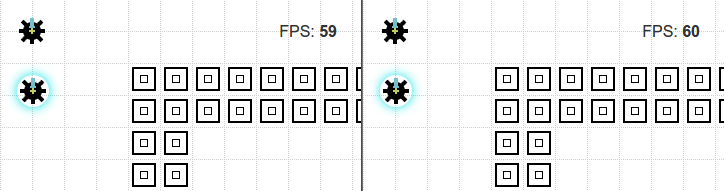
\includegraphics[width=0.9\linewidth]{lag-comp-action-f1}}\\
    \vspace{10pt}
    \raisebox{42pt}{\emph{f\textsubscript{2}}\hspace{5pt}} \fbox{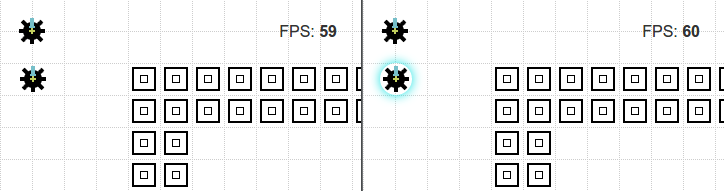
\includegraphics[width=0.9\linewidth]{lag-comp-action-f2}}\\
    \vspace{10pt}
    \raisebox{42pt}{\emph{f\textsubscript{3}}\hspace{5pt}} \fbox{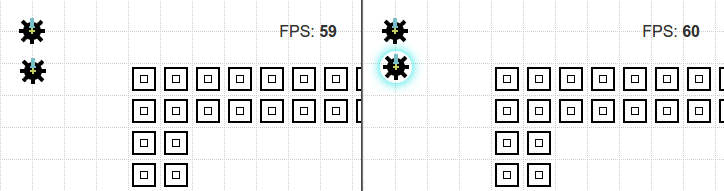
\includegraphics[width=0.9\linewidth]{lag-comp-action-f3}}\\
    \vspace{10pt}
    \raisebox{42pt}{\emph{f\textsubscript{4}}\hspace{5pt}} \fbox{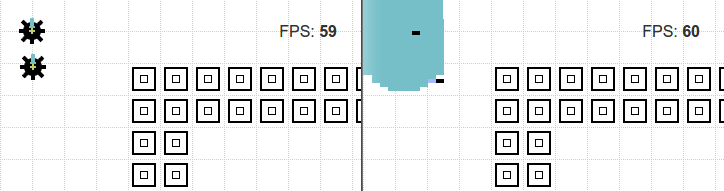
\includegraphics[width=0.9\linewidth]{lag-comp-action-f4}}\\
    \vspace{10pt}
    \raisebox{42pt}{\emph{f\textsubscript{5}}\hspace{5pt}} \fbox{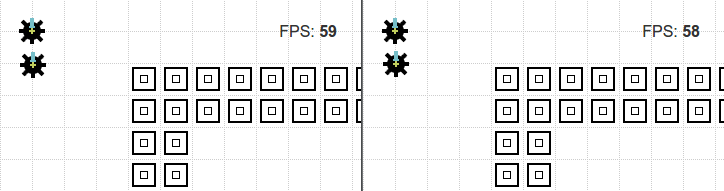
\includegraphics[width=0.9\linewidth]{lag-comp-action-f5}}
    \caption{#1}
    \label{lagCompInAction}
  \end{figure}
}


